% ---------------------------------------------------------------------------
% Shared body for the IEEE (IEEEtran) and Springer (llncs) versions.
% Every numerical result is a macro generated from the simulation output
% (numbers.tex, written by make_numbers.py from results/tables/*.csv).
% ---------------------------------------------------------------------------

\section{Introduction}\label{sec:intro}
Electricity used for space cooling in India rose by about a fifth between 2019 and
2022, and space cooling now accounts for roughly a tenth of national power demand
\cite{iea2023}. Much of this load comes from apartments, most of which are still
cooled by split air conditioners with on/off thermostats. Such a thermostat ignores
time-of-day (ToD) prices and the heat stored in a reinforced-concrete roof slab. It
also has no way to coordinate a variable-refrigerant-flow (VRF) unit with an
evaporative pre-cooler and a fresh-air system. In Pune the task changes with the
season. The composite climate has a dry pre-monsoon with afternoon peaks near
41\,$^\circ$C, a humid monsoon dominated by latent and ventilation loads, and a winter
that needs no cooling at all.

Model predictive control (MPC) handles this kind of problem by optimizing future inputs
over a forecast horizon with a building model \cite{drgona2020,afram2014}. Its savings
have been shown in simulation and in field tests \cite{oldewurtel2012,yao2021}. Deep reinforcement learning (DRL) learns a policy from
interaction with a simulator and needs no explicit model at run time
\cite{wei2017,wanghong2020,yu2021,sierla2022}. Hybrid schemes place a predictive layer
above feedback or learning \cite{arroyo2022}. Studies that compare these
methods often show one or more of three weaknesses. First, advanced controllers are often measured against
baselines that ignore indoor temperature or use different setpoints. Plant--model
mismatch, forecast error and repeated runs are also frequently left out, so results are
hard to reproduce \cite{blum2021,wangdong2024}. Second, few Indian residential
case studies combine typical-year weather, the national comfort range, ToD tariffs and
locally installed equipment \cite{manu2016}. Third, thermal control and indoor air
quality (IAQ) are rarely studied together, even though ventilation and filtration
choices change both cooling energy and exposure \cite{belias2022}.

We address these gaps with a year-long benchmark of five controllers on one openly
released model of a 95\,m$^2$ top-floor apartment in Pune. The paper makes four
contributions:
\begin{itemize}
\item a reproducible MATLAB/Octave/Simulink plant comprising an exactly discretized
      two-node-per-zone RC network, an inverter VRF with part-load and latent
      behaviour, indirect evaporative cooling (IEC), a dedicated outdoor-air system
      (DOAS) with energy recovery, and moisture, CO$_2$ and PM$_{2.5}$ balances;
\item a like-for-like comparison of a thermostat, SIMC-tuned PID, economic MPC (E-MPC),
      a shielded double deep Q-network (DQN) and a hybrid E-MPC/PI controller, all
      subject to plant--model mismatch, sensor noise and forecast error, sharing one
      comfort schedule and replicated over five seeds;
\item a discomfort metric that counts only cooling-induced overcooling, since the
      dwelling has no heating and weather-driven cold lies outside every controller's
      authority;
\item tests of the mechanisms behind the results, namely perfect-information, back-off
      and layer-removal ablations, three tariff structures including the actual utility
      tariff, and a 40-sample variation of eleven assumed inputs.
\end{itemize}
Section~\ref{sec:related} reviews related work, Section~\ref{sec:method} describes the
plant and controllers, Section~\ref{sec:results} presents the experiments, and
Section~\ref{sec:conclusion} concludes.

\section{Related Work}\label{sec:related}
\subsection{Model predictive control of buildings}
Reviews of MPC for buildings cover problem formulation, model classes and solvers
\cite{afram2014,drgona2020}, and HVAC-specific applications with their reported savings
\cite{yao2021}. Oldewurtel \emph{et al.} \cite{oldewurtel2012} quantified the value of
weather forecasts in a large factorial study and proposed a stochastic MPC that
accounts for forecast uncertainty. These controllers usually rely on reduced-order RC models,
which never match the building exactly. Integrating disturbance states, estimated with a
Kalman filter, remove the resulting steady-state offset \cite{pannocchia2003}. Economic
MPC with a tariff-weighted cost suits ToD pricing, although its comfort depends on how
close to the comfort bound it is allowed to operate; Section~\ref{sec:sens} examines
this trade-off.

\subsection{Reinforcement learning for HVAC}
Deep Q-networks \cite{mnih2015} and their double-estimator variant
\cite{vanhasselt2016} are common choices in DRL studies of HVAC control. Wei
\emph{et al.} \cite{wei2017}, for example, used a DQN to set airflow in a multi-zone
building.
Later reviews \cite{wanghong2020,yu2021,sierla2022} point to long and data-hungry
training, weak safety guarantees and poor generalization as the main obstacles to
deployment. Experimental comparisons of model-free algorithms also report a strong
sensitivity to the random seed and to reward design \cite{biemann2021}. We adopt
shielding, which enforces safety constraints by overriding unsafe actions before they
reach the plant \cite{alshiekh2018}.

\subsection{Comparative studies and benchmarking}
Few studies compare MPC, DRL and conventional feedback on one plant with the same
information available to each controller. Arroyo \emph{et al.} \cite{arroyo2022} combined MPC with RL
and compared the result with both parent methods, and Wang and Dong \cite{wangdong2024}
reported a long-term experimental comparison of advanced HVAC controls. BOPTEST
\cite{blum2021} provides standardized emulators and performance indicators, so that
results from different studies can be compared directly. Reduced-order models are
usually cross-checked against a detailed engine such as EnergyPlus \cite{crawley2001}.

\subsection{Indian residential context}
Field studies across Indian climate zones produced the India Model for Adaptive Comfort
(IMAC) \cite{manu2016}. For air-conditioned buildings the 2005 National Building Code
prescribes a static summer range of 23--26\,$^\circ$C \cite{nbc2005}, and the
residential energy code, Eco-Niwas Samhita, limits the roof U-value \cite{ens2018}.
The ventilation rate in this study follows ASHRAE~62.2 \cite{ashrae622}. Filtration has
a strong effect on indoor PM$_{2.5}$ \cite{belias2022}, for which the WHO guideline
\cite{who2021} and the Indian NAAQS \cite{cpcb2009} set limits. Residential tariffs in
Maharashtra are set by the state regulator \cite{merc}, and the Central Electricity
Authority publishes the grid emission factor \cite{cea}.

\section{Methodology}\label{sec:method}
\subsection{Case-study dwelling and weather}
The case is a 95\,m$^2$ top-floor three-bedroom flat (18.53$^\circ$N, 73.85$^\circ$E)
with three conditioned zones: a master bedroom (30\,m$^2$), a living room (45\,m$^2$)
and a second bedroom (20\,m$^2$). Walls are 200\,mm aerated concrete
($U=0.75$\,W\,m$^{-2}$K$^{-1}$). The 150\,mm concrete roof slab is insulated to
$U=1.2$\,W\,m$^{-2}$K$^{-1}$, the Eco-Niwas Samhita limit \cite{ens2018}. Windows are
double glazed ($U=2.8$\,W\,m$^{-2}$K$^{-1}$, SHGC 0.55) at a window-to-wall ratio of
0.20, with overhang shading. Weather comes from the ISHRAE typical year for
Pune \cite{ishrae}, with hourly records interpolated to a 15-min step. Dry-bulb
temperature ranges from 4.9 to 41.0\,$^\circ$C, and monsoon relative humidity stays above
80\,\% from July to October. Four occupants follow weekday and weekend schedules;
lighting, equipment and cooking gains follow fixed profiles.

\begin{figure*}[!t]\centering
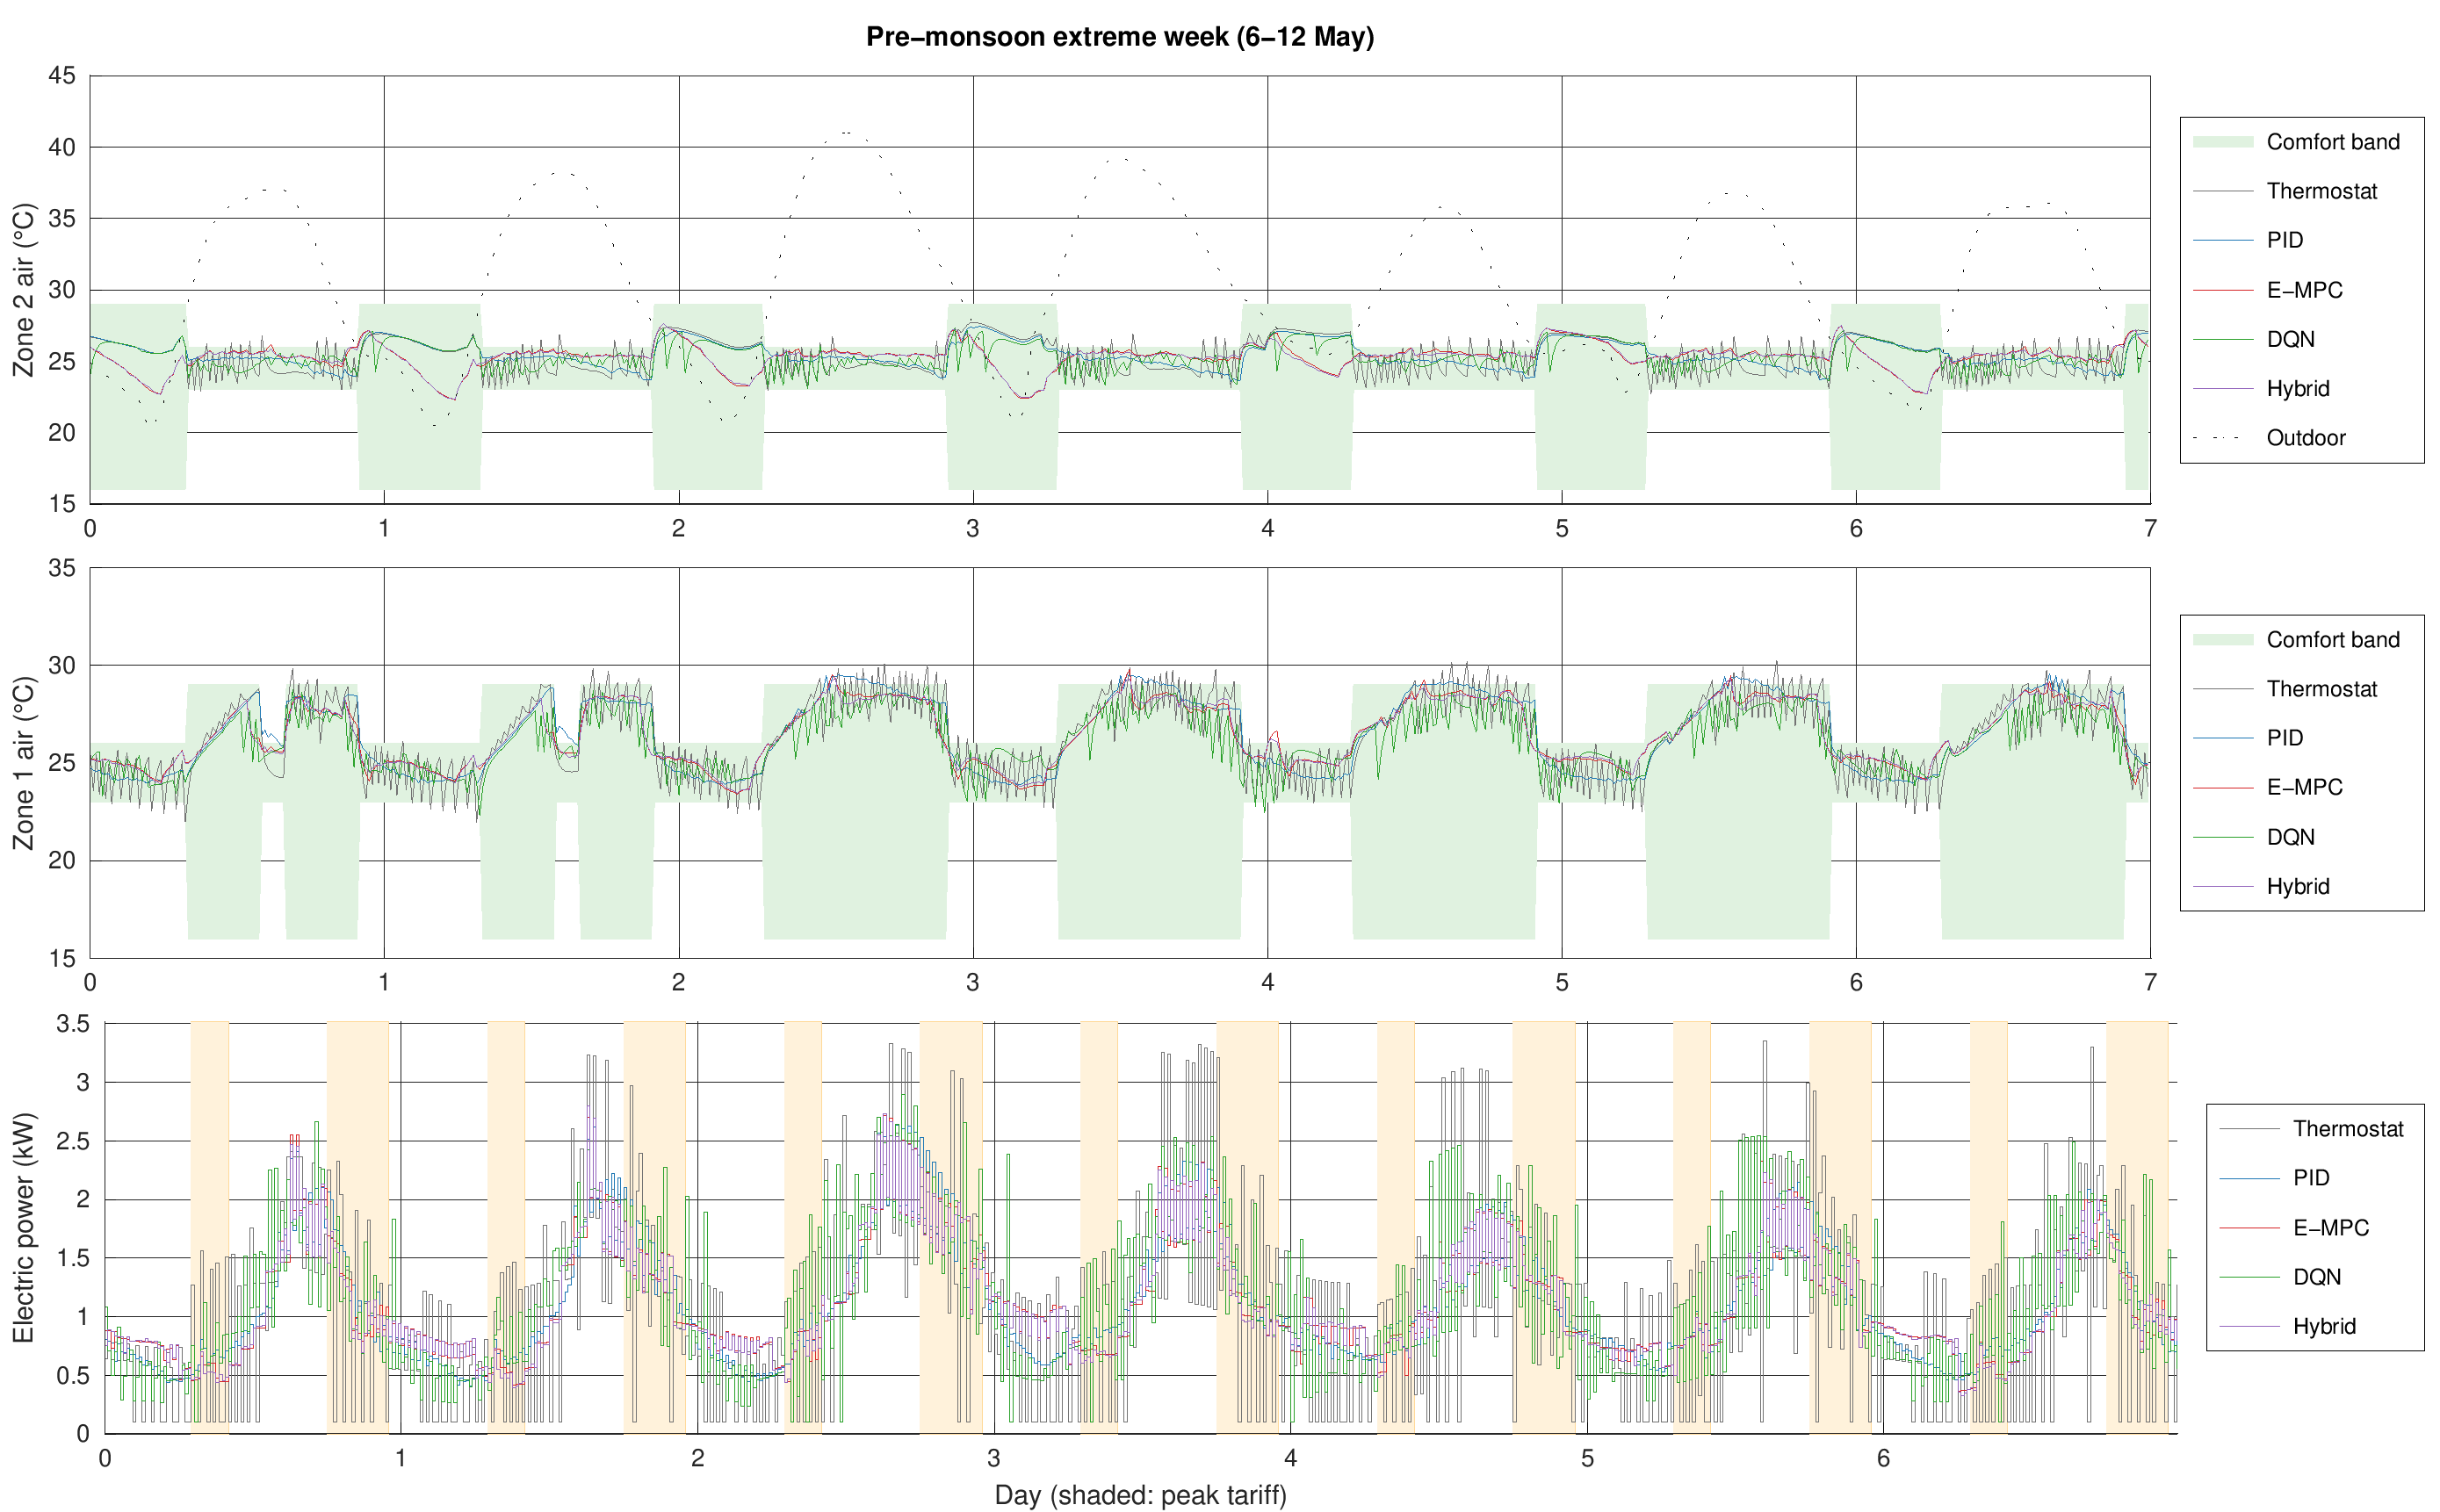
\includegraphics[width=0.82\textwidth]{Fig02a_week_1.png}
\caption{Extreme pre-monsoon week (6--12 May), seed 1. Top: Zone~2 air temperature,
comfort band (shaded) and outdoor temperature. Middle: Zone~1. Bottom: total electric
power, with peak-tariff hours shaded.}\label{fig:week}
\end{figure*}

\subsection{Thermal model}
Each zone $z\in\{1,2,3\}$ has an air node $T_{a,z}$ and a thermal-mass node $T_{m,z}$:
\begin{align}
C_{a,z}\dot T_{a,z} ={}& H_{am,z}(T_{m,z}-T_{a,z}) \nonumber\\
  &+ (UA_{g,z}+H_{inf,z})(T_o-T_{a,z}) \nonumber\\
  &+ \textstyle\sum_{j\neq z} H_{zj}(T_{a,j}-T_{a,z}) + f_s Q_{sol,z} \nonumber\\
  &+ f_c Q_{int,z} + Q_{vent,z} - Q_{c,z}, \label{eq:air}\\
C_{m,z}\dot T_{m,z} ={}& H_{am,z}(T_{a,z}-T_{m,z}) \nonumber\\
  &+ UA_{w,z}(T_{sa,w,z}-T_{m,z}) \nonumber\\
  &+ UA_{r,z}(T_{sa,r}-T_{m,z}) \nonumber\\
  &+ (1-f_s)Q_{sol,z} + (1-f_c)Q_{int,z}. \label{eq:mass}
\end{align}
Here $T_{sa}$ denotes sol-air temperature, $Q_{sol}$ is transmitted solar gain (a
fraction $f_s=0.3$ reaches the air node), $Q_{int}$ is internal gain with convective
fraction $f_c=0.6$, $Q_{vent}$ is the sensible effect of DOAS and IEC supply air, and
$Q_c$ is the sensible cooling delivered by the indoor unit. With
$x=[T_{a,1..3},T_{m,1..3}]^\top$, $u=[Q_{c,1..3}]^\top$ and disturbance vector $d$, the
model $\dot x=Ax+Bu+Ed$ is discretized exactly under a zero-order hold with
$\Delta t=900$\,s:
\begin{equation}
\begin{bmatrix}A_d & B_d & E_d\end{bmatrix}
=\begin{bmatrix}I&0&0\end{bmatrix}
\exp\!\left(\begin{bmatrix}A&B&E\\0&0&0\end{bmatrix}\Delta t\right).
\label{eq:zoh}
\end{equation}
The update $x_{k+1}=A_dx_k+B_du_k+E_dd_k$ is unconditionally stable and agrees with
fine-step RK4 integration to $10^{-12}$\,K over 24\,h. Modal time constants are
0.35--0.43\,h for the air nodes and 25--36\,h for the mass nodes.

The model-based controllers use nominal parameters, but the simulated plant departs
from them: mass capacitance is scaled by 0.85, air capacitance and envelope
conductance by 1.10, solar gain by 1.10 and internal gain by 1.15. Every controller
receives zone temperatures corrupted by Gaussian noise ($\sigma=0.1$\,K).

\subsection{HVAC equipment}
An 11\,kW inverter VRF outdoor unit serves indoor units of 3.5, 5.0 and 2.5\,kW. Its
capacity derates by 0.8\,\%\,K$^{-1}$ above 35\,$^\circ$C, and its energy input ratio
rises by 2.5\,\%\,K$^{-1}$ from a rated COP of 3.8. Part-load behaviour follows
$\mathrm{EIR}(\mathrm{PLR})=0.08+0.62\,\mathrm{PLR}+0.30\,\mathrm{PLR}^2$ down to
20\,\% modulation, below which the unit cycles with degradation coefficient 0.25. The
sensible heat ratio is 0.75 while the indoor humidity ratio exceeds the coil apparatus
dew point and 1 otherwise, and the unit operates for outdoor temperatures of
10--50\,$^\circ$C.

The IEC supplies product air at $T_{sup}=T_o-0.8(T_o-T_{wb})$ without adding moisture.
A rule common to all controllers enables it when outdoor air is hot and dry, cooling is
requested, and $T_{sup}$ is at least 2\,K below the mean zone temperature. The DOAS
ventilates continuously at the ASHRAE~62.2 rate of 28\,L\,s$^{-1}$ \cite{ashrae622}
through an energy-recovery ventilator (sensible effectiveness 0.70, latent 0.60), a
MERV-13 filter, and a dehumidifying coil that runs only when indoor humidity exceeds
0.0115\,kg\,kg$^{-1}$.

\subsection{Moisture and indoor air quality}
Indoor humidity ratio $W$, CO$_2$ concentration $C$ and PM$_{2.5}$ concentration $P$
obey well-mixed balances over the conditioned volume $V$. For CO$_2$ and PM$_{2.5}$,
\begin{align}
V\dot C &= F_{out}(C_o-C)+n_{occ}\,g_{\mathrm{CO_2}},\label{eq:co2}\\
V\dot P &= P_o\big(pF_{inf}+(1-\eta_d)F_d\big) + S_{PM} \nonumber\\
        &\quad -\big(F_{out}+\eta_r F_r+kV\big)P, \label{eq:pm}
\end{align}
where $p=0.8$ is the infiltration penetration factor, $\eta_d$ and $\eta_r$ are the
DOAS and HEPA recirculation filter efficiencies, $k=0.5$\,h$^{-1}$ is the deposition
rate, and $S_{PM}$ collects cooking and background emissions. The humidity balance has
the same form. Each balance is linear, with coefficients held constant over a step, so it
can be integrated exactly as $y_{k+1}=y_\infty+(y_k-y_\infty)e^{-\kappa\Delta t}$, which remains
stable for any removal rate $\kappa$.

\begin{table*}[!t]\centering
\caption{Annual results, mean $\pm$ 95\,\% CI over five seeds. Discomfort counts
occupied overheating plus cooling-induced overcooling; $\Delta$cost is relative to the
thermostat.}\label{tab:main}
\resizebox{\textwidth}{!}{% generated by aggregate_results.m -- mean +/- 95% CI over 5 seeds
\begin{tabular}{lrrrrrrr}
\toprule
Controller & Energy (kWh) & Cost (INR) & $\Delta$cost & Disc. (K\,h) & Acc. (\%) & RMSE (K) & Peak (kW)\\
\midrule
Thermostat & 5028 $\pm$ 1 & 36950 $\pm$ 8 & -- & 1101.5 $\pm$ 3.2 & 82.7 $\pm$ 0.1 & 1.17 $\pm$ 0.00 & 3.38 $\pm$ 0.01\\
PID & 5403 $\pm$ 0 & 39460 $\pm$ 3 & +6.8\% & 315.3 $\pm$ 0.5 & 94.8 $\pm$ 0.0 & 0.75 $\pm$ 0.00 & 2.69 $\pm$ 0.04\\
E-MPC & 5243 $\pm$ 3 & 38306 $\pm$ 26 & +3.7\% & 250.6 $\pm$ 2.2 & 95.7 $\pm$ 0.0 & 0.99 $\pm$ 0.00 & 2.78 $\pm$ 0.07\\
DQN & 5273 $\pm$ 112 & 38799 $\pm$ 682 & +5.0\% & 259.2 $\pm$ 53.8 & 94.3 $\pm$ 0.8 & 0.90 $\pm$ 0.04 & 3.32 $\pm$ 0.07\\
Hybrid & 5198 $\pm$ 1 & 38005 $\pm$ 14 & +2.9\% & 185.1 $\pm$ 1.1 & 96.1 $\pm$ 0.0 & 0.99 $\pm$ 0.00 & 2.78 $\pm$ 0.10\\
\bottomrule
\end{tabular}
}
\end{table*}

\subsection{Control strategies}
All controllers act on the same plant and share one comfort schedule. Occupied zones
use the 23--26\,$^\circ$C band \cite{nbc2005} with a 24.5\,$^\circ$C setpoint;
unoccupied zones use 16--29\,$^\circ$C with a 28.5\,$^\circ$C setpoint.

\emph{Thermostat.} Each indoor unit runs at full capacity once its zone exceeds the
setpoint by 0.5\,K and stops 0.5\,K below it.

\emph{PID.} Each zone has its own PI loop with a filtered derivative, back-calculation
anti-windup and output limits $[0,\bar u_z]$. The loops are tuned with the SIMC rules
\cite{skogestad2003} for an integrating approximation of each zone response, which give
$K_c=1/(k'(\tau_c+\theta))$ and $T_i=\min(\tau,4(\tau_c+\theta))$ with
$\tau_c=15$\,min.

\emph{Economic MPC.} Every hour the controller solves
\begin{multline}
\min_{U}\;\sum_{h=1}^{N_h}\sum_{z}
   \frac{\pi_h\,\mathrm{EIR}_T(\hat T_{o,h})}{\mathrm{COP}_r\,\mathrm{SHR}}\,U_{h,z}
 + \lambda\sum_h\|U_h-U_{h-1}\|^2\\
 +\rho\sum_{j,z}\Big(\big[\hat T_{a,z,j}-\overline T_{z,j}+\delta\big]_+^2\\
 +\big[\underline T_{z,j}+\delta-\hat T_{a,z,j}\big]_+^2\Big)
\label{eq:empc}
\end{multline}
subject to $0\le U_{h,z}\le\bar u_z$ and
$\sum_z U_{h,z}\le\mathrm{SHR}\cdot Q_{cap}(\hat T_{o,h})$. Inputs are held
constant within each hour over a horizon of $N_h=24$\,h, and $\pi_h$ is the ToD price.
Comfort enters as a soft penalty with weight $\rho=50$\,INR\,K$^{-2}$ and back-off
$\delta=0.5$\,K, while $\lambda=0.05$ penalizes input moves. Predictions start from a
steady-state Kalman filter augmented with three integrating disturbance states
\cite{pannocchia2003}. The weather forecasts carry a dry-bulb error that grows as
$0.15\sqrt{h}$\,K (capped at 2\,K) and a 10\,\% solar error. The convex problem is solved by FISTA \cite{beck2009} with an exact projection
onto the box-and-capacity set and 120 warm-started iterations.

\emph{DQN.} A parameter-shared double DQN \cite{mnih2015,vanhasselt2016} acts on each
zone every 15\,min, choosing among five capacity levels (0--100\,\% in steps of
25\,\%). Its 15 input features are the temperature error, outdoor temperature and its
3-h forecast change, time-of-day and day-of-year encodings, tariff, occupancy, setpoint,
previous action and a one-hot zone index. The reward is the negative sum of the zone's
ToD cost, the squared band violation weighted by $\beta=\rho$, and a switching penalty.
The 64--64 ReLU network is trained with Huber loss, Adam and Polyak target updates over
200 fourteen-day episodes, each drawn from a randomly perturbed copy of the typical year.
The checkpoint is chosen by its greedy return on five fixed validation fortnights. A
safety shield is active during both training and deployment \cite{alshiekh2018}: it
blocks cooling near the lower band and enforces at least 50\,\% capacity when an
occupied zone is 0.5\,K above the upper band. The replay buffer stores the agent's
\emph{proposed} action, and a penalty is added each time the shield overrides it.

\emph{Hybrid.} The E-MPC supplies an hourly feed-forward $U_h$ and a 15-min reference
$\hat T_a$, which a PI layer with half the SIMC gain tracks:
\begin{equation}
u_k=\mathrm{sat}\big(U_h+K_he_k+v_k\big),\qquad e_k=T^{meas}_{a,k}-\hat T_{a,k},
\label{eq:hyb}
\end{equation}
with $v_k$ a leaky integral state. A safety override enforces $u_z\ge0.8\,\bar u_z$
whenever an occupied zone exceeds its band by 0.5\,K. Algorithm~\ref{alg:hybrid} gives
one control step.

\begin{algorithm}[t]
\caption{Hybrid controller, one 15-min step for zone $z$}\label{alg:hybrid}
\begin{algorithmic}[1]
\IF{start of an hour}
  \STATE update Kalman estimate $\hat x$ and disturbance $\hat d$
  \STATE solve \eqref{eq:empc} by FISTA; store $U_h$ and reference $\hat T_a$
\ENDIF
\STATE $e_k\leftarrow T^{meas}_{a,z,k}-\hat T_{a,z,k}$
\IF{$U_{h,z}>0$ \OR $T^{meas}_{a,z,k}>\overline T_{z,k}-\delta$}
  \STATE $v_k\leftarrow \gamma v_{k-1}+(K_h\Delta t/T_i)\,e_k$ \COMMENT{PI active}
\ELSE
  \STATE $v_k\leftarrow \gamma v_{k-1}$ \COMMENT{integrator leaks}
\ENDIF
\STATE $u_{z,k}\leftarrow\mathrm{sat}_{[0,\bar u_z]}(U_{h,z}+K_he_k+v_k)$
\IF{zone occupied \AND $T^{meas}_{a,z,k}>\overline T_{z,k}+0.5$}
  \STATE $u_{z,k}\leftarrow\max(u_{z,k},0.8\,\bar u_z)$ \COMMENT{safety override}
\ENDIF
\STATE back-calculate $v_k$ if $u_{z,k}$ saturated
\end{algorithmic}
\end{algorithm}

\subsection{Metrics}
The energy and cost metrics are annual electricity by end use, cost under a three-tier
ToD tariff (INR 5.20/7.15/8.95 per kWh), 15-min peak demand, the share of VRF energy
used in peak hours, and operational CO$_2$ emissions at the national grid factor of
0.727\,kgCO$_2$ per kWh \cite{cea}. The three-tier tariff is hypothetical and does not
correspond to a published utility schedule; Section~\ref{sec:sens} evaluates the
utility's actual residential structure \cite{merc}. Occupied discomfort $K_h$ (K\,h) sums overheating above the band
and \emph{cooling-induced} overcooling below $\min(\underline T,T^{free})$, where
$T^{free}$ comes from a free-floating run without cooling. We also report humid
hours (RH above 70\,\%) and CO$_2$ and PM$_{2.5}$ exposure.

\section{Experimental Setup and Results}\label{sec:results}
\subsection{Setup}
Each controller was simulated over the full typical year at a 15-min step (35{,}040
steps). The main study uses five seeds. A seed fixes the sensor noise and forecast
errors and, for the DQN, the training run. Means are reported with 95\,\%
$t$-intervals. Paired comparisons use seed-1 daily totals with a 7-day moving-block
bootstrap and the Wilcoxon signed-rank test. We ran the code in both GNU Octave 10.3
and MATLAB R2024a; noise-free trajectories agree to within $10^{-12}$. A Simulink
wrapper of the same plant and controllers reproduced the MATLAB results exactly in a
seven-day test.


\begin{figure*}[!t]\centering
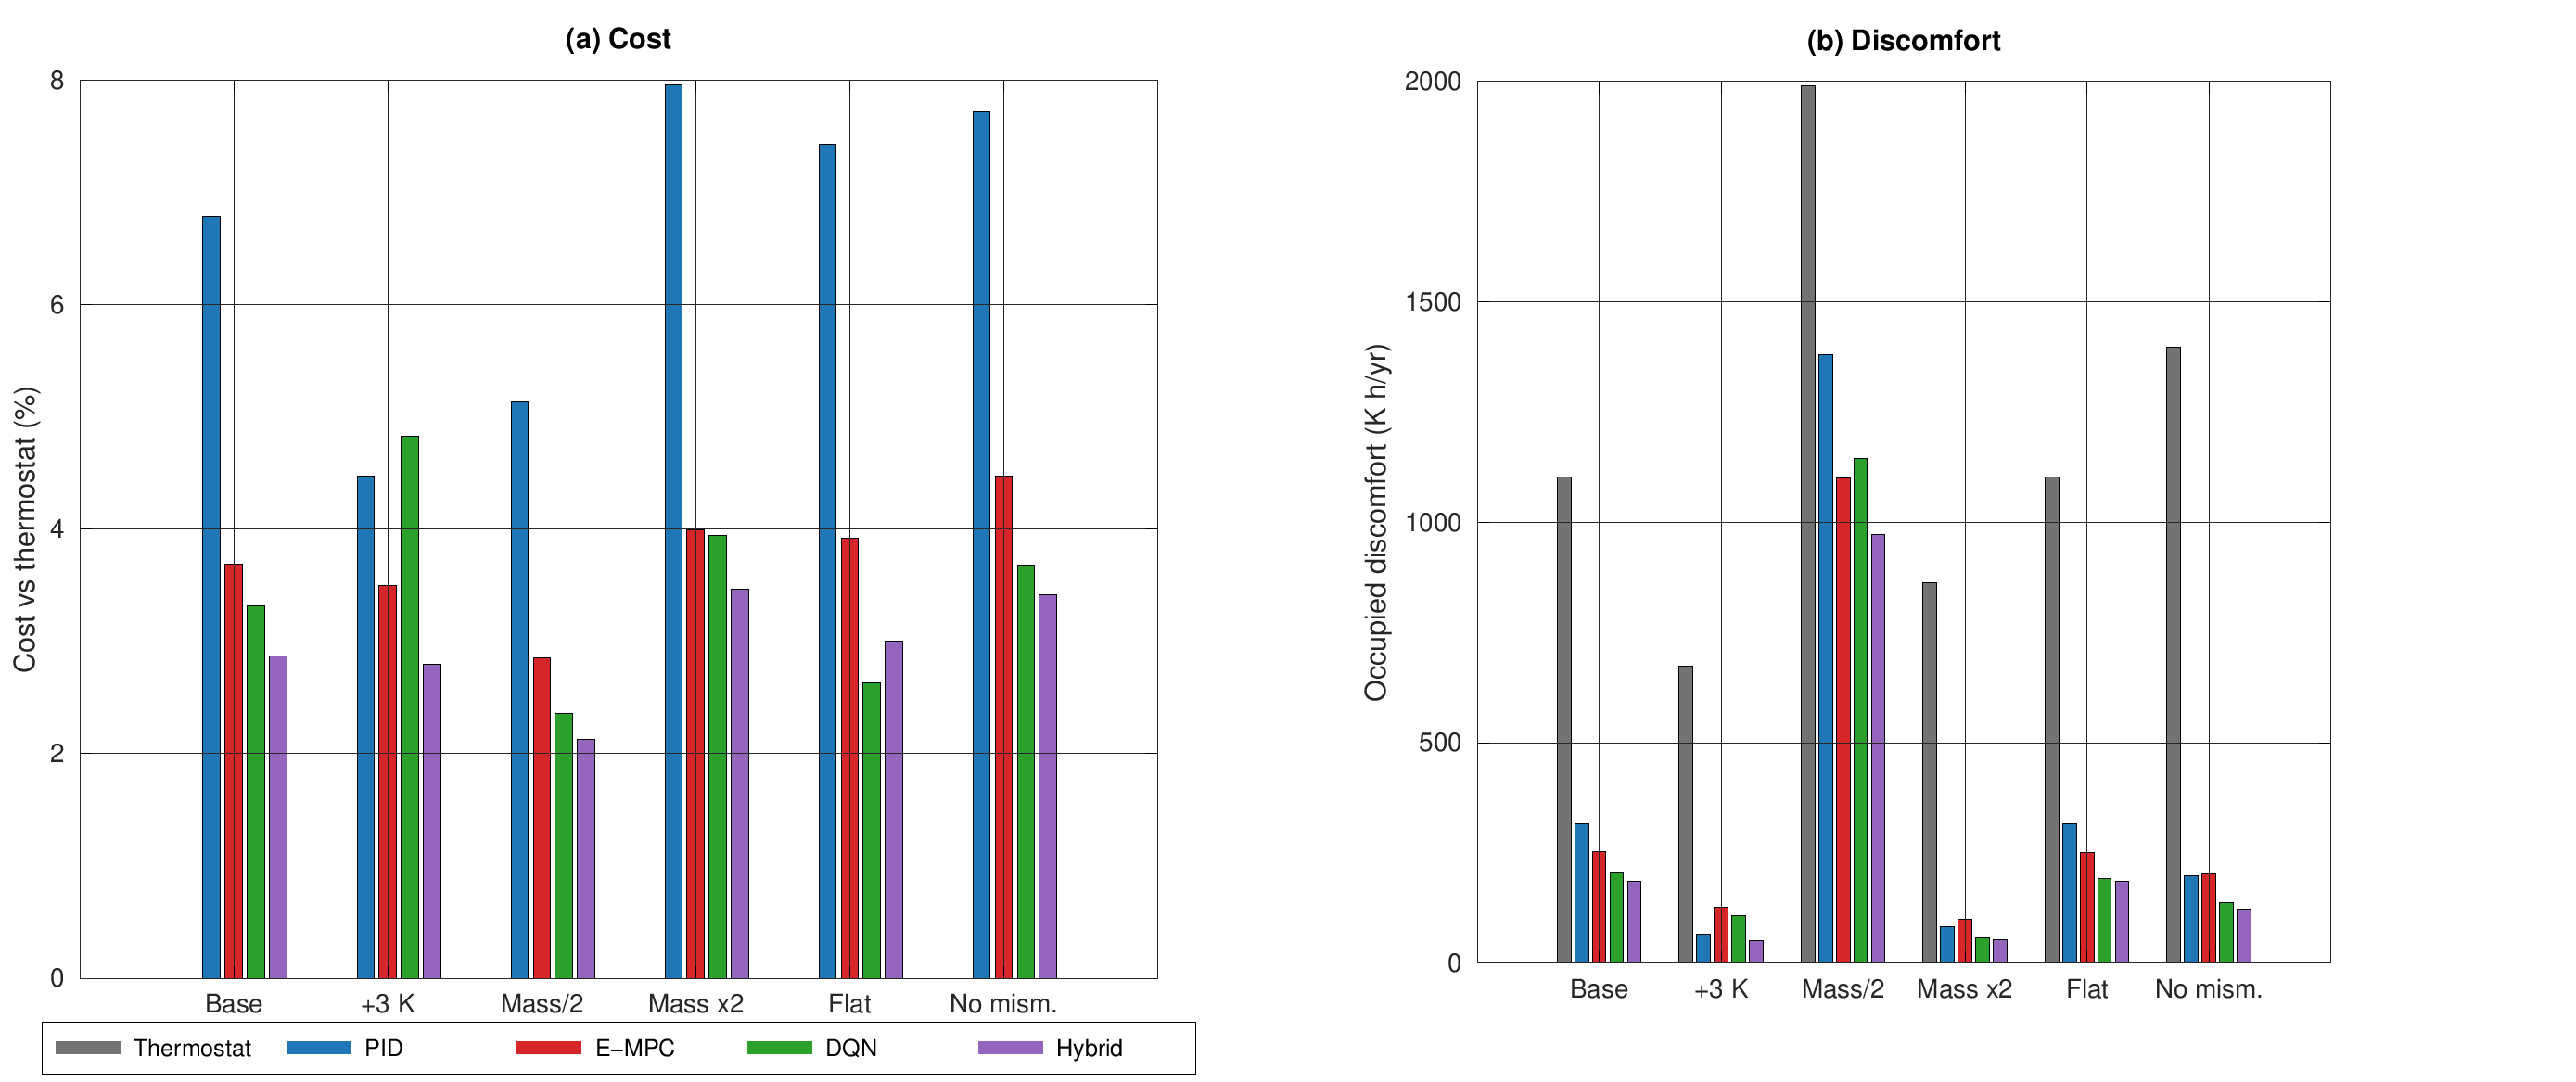
\includegraphics[width=0.82\textwidth]{Fig08_sensitivity.png}
\caption{Sensitivity of (a) annual cost relative to the thermostat and (b) occupied
discomfort across scenarios (seed 1).}\label{fig:sens}
\end{figure*}

\subsection{Annual cost, energy and comfort}
Table~\ref{tab:main} and Fig.~\ref{fig:pareto} summarize the annual results, and
Fig.~\ref{fig:week} shows the extreme week. The thermostat is the cheapest controller
(INR~\CostTh) but has the largest discomfort (\KhTh\,K\,h) and the fewest acceptable
occupied hours (\AccTh\,\%). Overcooling makes up \KhColdTh\,K\,h of that total. Each unit runs at full
output until its zone is 0.5\,K below setpoint, and with a 25-min air time constant the
zone keeps cooling to well below 23\,$^\circ$C. The thermostat also starts
the compressor \StartsTh{} times a year, compared with \StartsHyb{} for the Hybrid.

The four modulating controllers reduce discomfort by 71--83\,\% relative to the
thermostat at a cost penalty of 2.9--6.8\,\%. The Hybrid is best on both criteria
(INR~\CostHyb, \KhHyb\,K\,h, \AccHyb\,\% acceptable). It is \RelHybPidCost\,\% cheaper
than PID with \RelHybPidKh\,\% less discomfort, and \RelHybMpcCost\,\% cheaper than
E-MPC with \RelHybMpcKh\,\% less discomfort. E-MPC in turn undercuts PID on cost
(INR~\CostMpc{} against \CostPid) at lower discomfort (\KhMpc{} against \KhPid\,K\,h).
The shielded DQN matches E-MPC on discomfort (\KhDqn\,K\,h) and falls between PID and
E-MPC on cost. Its results also vary far more from seed to seed than those of any other
controller (cost $\pm$\CostDqnCI{} INR, discomfort $\pm$\KhDqnCI\,K\,h).


\begin{figure}[t]\centering
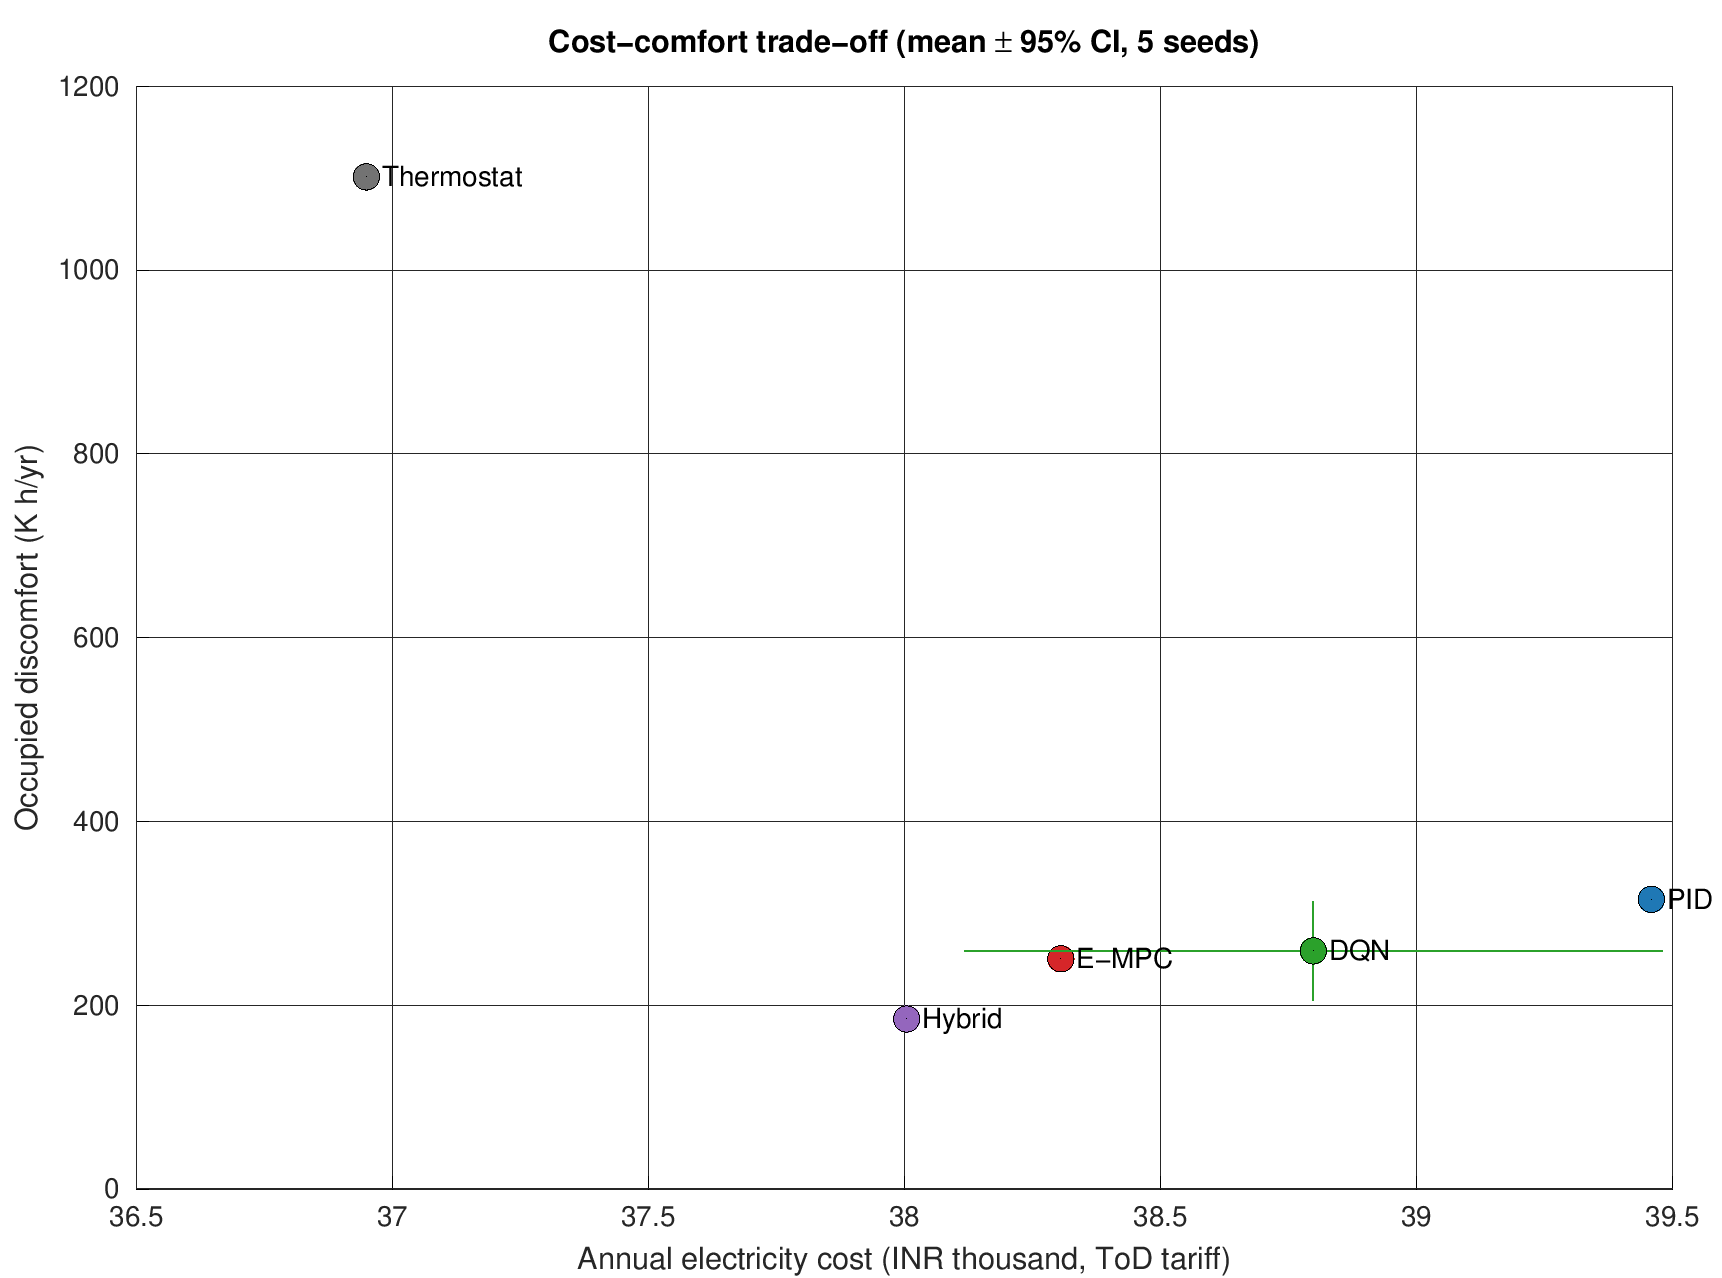
\includegraphics[width=0.92\linewidth]{Fig05_pareto.png}
\caption{Annual ToD cost versus occupied discomfort (mean $\pm$ 95\,\% CI, five seeds).}
\label{fig:pareto}
\end{figure}

The paired daily tests support these differences. Relative to PID, the Hybrid changes
annual cost by INR~$\PairHybridPidCost${} [$\PairHybridPidCostLo$, $\PairHybridPidCostHi$]
and discomfort by $\PairHybridPidKh$\,K\,h [$\PairHybridPidKhLo$, $\PairHybridPidKhHi$],
both with $p\PairHybridPidCostP$. Relative to E-MPC the changes are
INR~$\PairHybridMpcCost${} and $\PairHybridMpcKh$\,K\,h, again with $p\PairHybridMpcCostP$.
Between E-MPC and PID only the cost difference is significant; the discomfort
difference is not ($p=\PairMpcPidKhP$).

\subsection{Energy use and load shifting}
The VRF uses 61--65\,\% of annual electricity (Fig.~\ref{fig:energy}). About a
quarter goes to the DOAS, mostly for monsoon dehumidification; this is the largest load
that the thermal controllers do not govern. Monthly consumption peaks in May at 760--805\,kWh.


\begin{figure}[t]\centering
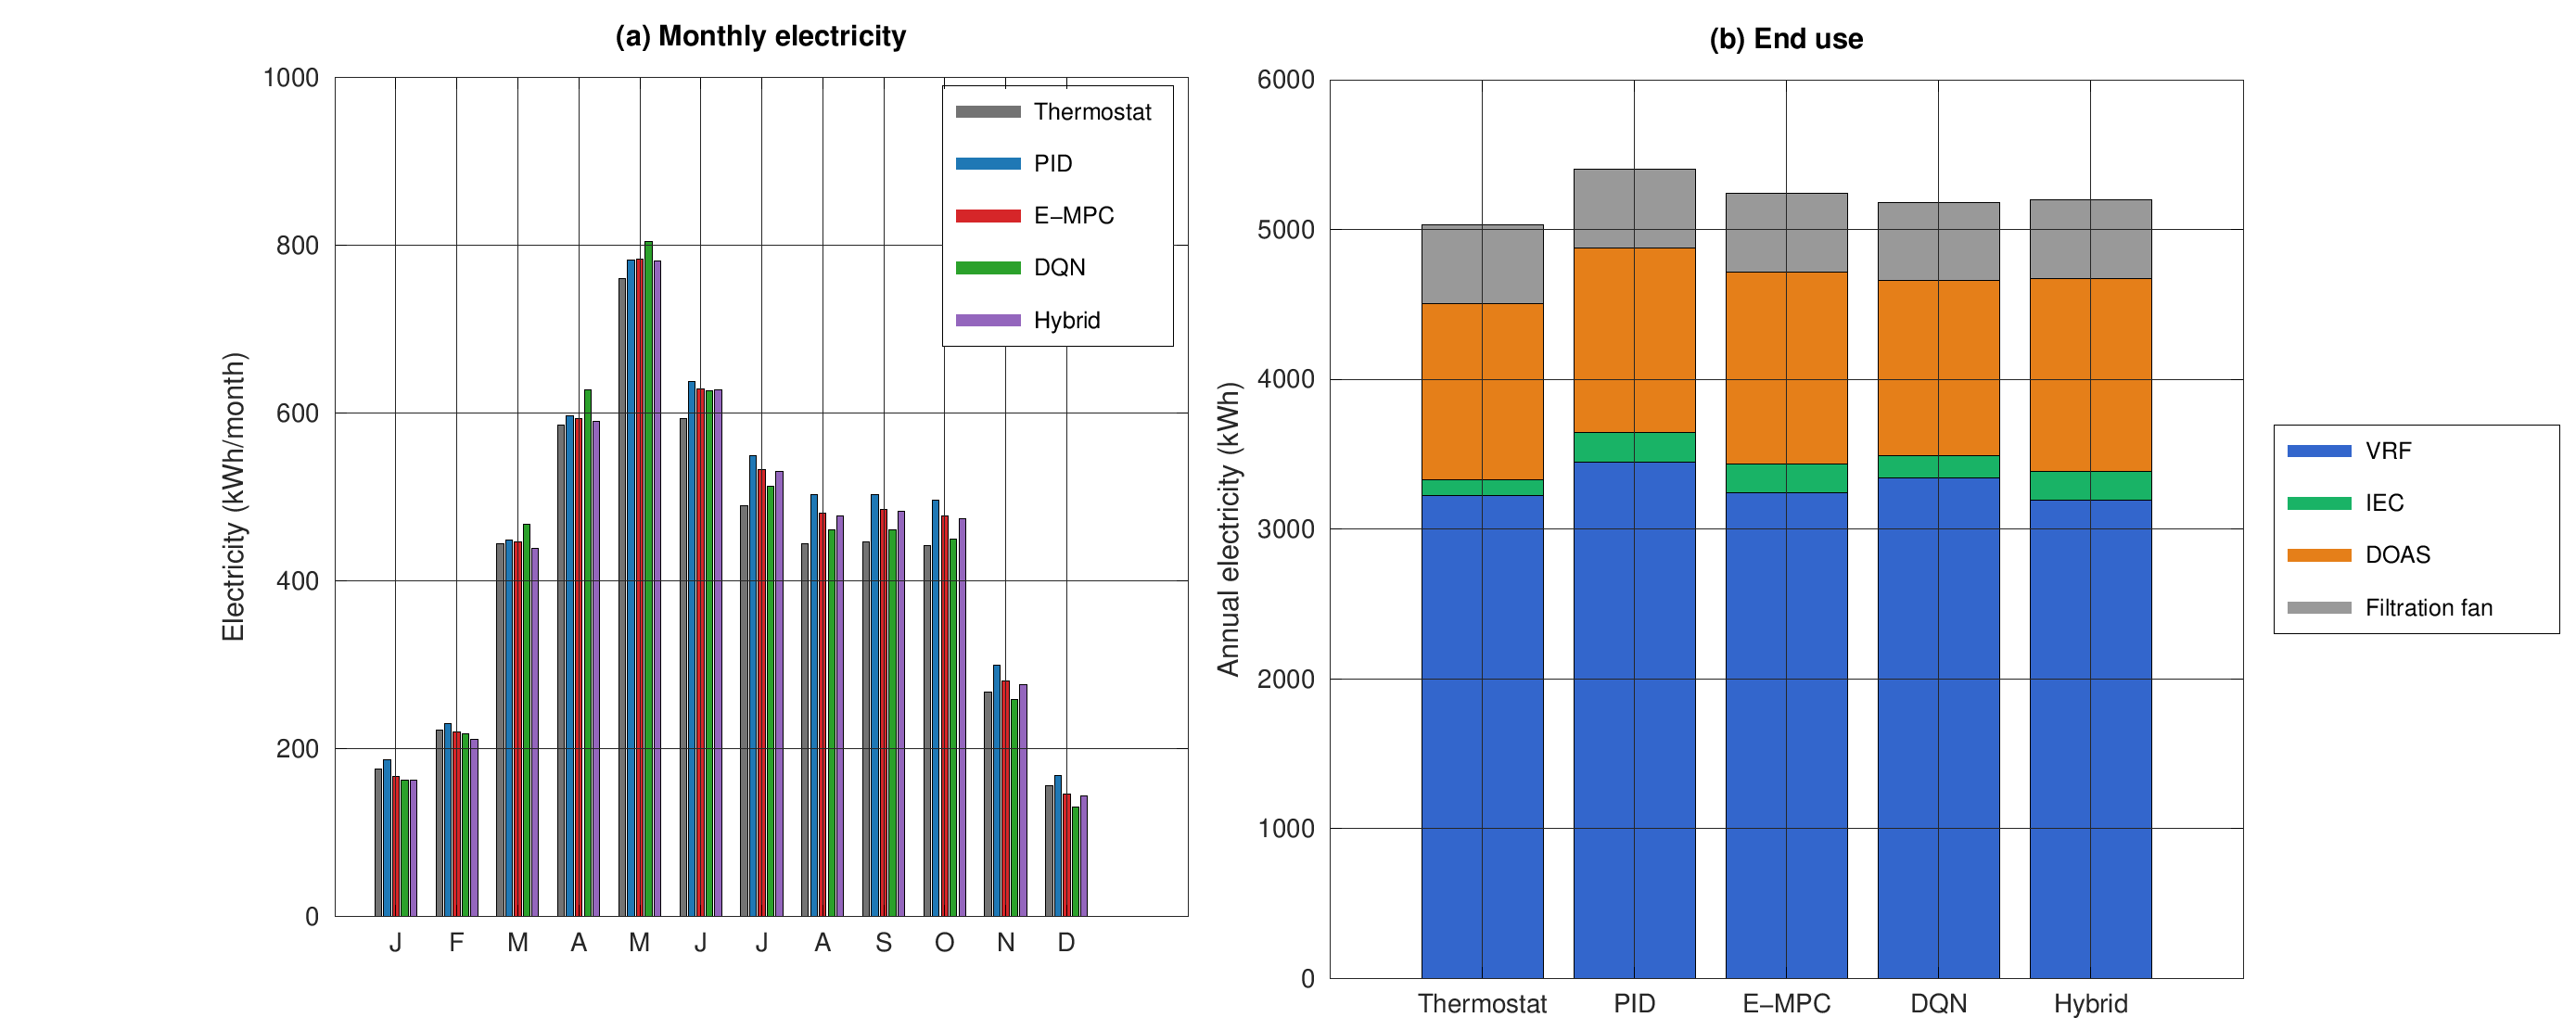
\includegraphics[width=\linewidth]{Fig03_energy.png}
\caption{(a) Monthly electricity and (b) annual end-use split, seed 1.}
\label{fig:energy}
\end{figure}

Fig.~\ref{fig:profile} shows the mean March--June profile of VRF power. E-MPC and Hybrid
pre-cool the thermal mass between 00:00 and 05:00 and draw less power in the late
morning. Even so, the share of VRF energy in peak-tariff hours is almost the same for
every controller (\PeakShareTh--\PeakShareDqn\,\%), and replacing the ToD tariff with a
flat one changes E-MPC energy use by less than 0.5\,\%. The predictive controllers save
mainly through temperature-aware efficiency and by operating near the upper comfort
bound; price arbitrage contributes little. Two features of the dwelling limit load
shifting. All of the peak-window cooling serves occupied zones, so it cannot be dropped
without discomfort, and the roof slab releases stored heat in the evening: mean
slab-to-air heat flow is about 2.5\,kW during 18:00--23:00, against 1.8\,kW during
10:00--16:00.

\begin{figure}[t]\centering
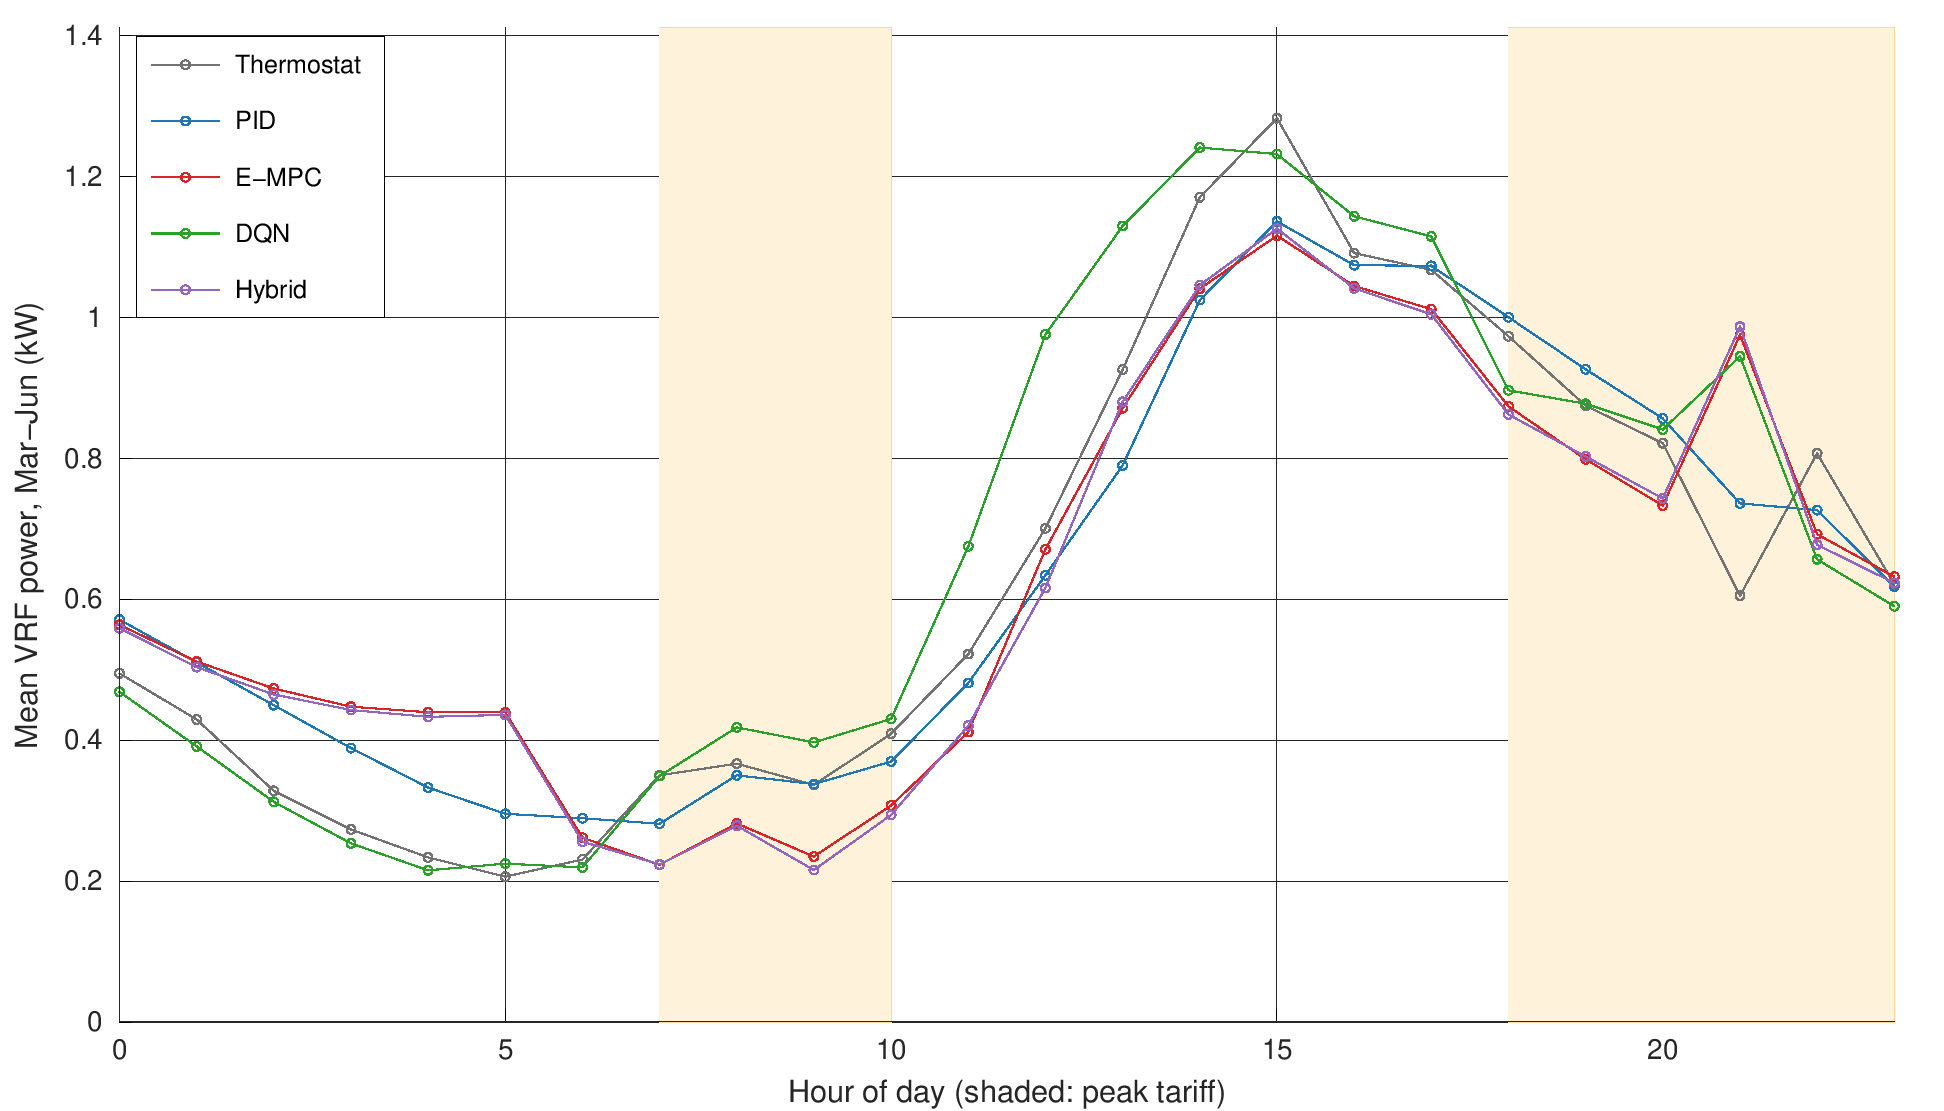
\includegraphics[width=0.95\linewidth]{Fig04_daily_profile.png}
\caption{Mean VRF power by hour, March--June, seed 1; peak-tariff hours shaded.}
\label{fig:profile}
\end{figure}

\subsection{Robustness, mechanisms and sensitivity}\label{sec:sens}
Table~\ref{tab:sens} and Fig.~\ref{fig:sens} give the single-seed robustness and
ablation results.

\emph{Heatwave.} With dry-bulb temperature raised by 3\,K all year, the Hybrid remains
best (INR~\SHeatCostHyb, \SHeatKhHyb\,K\,h), but PID's discomfort (\SHeatKhPid\,K\,h)
falls below that of E-MPC (\SHeatKhMpc\,K\,h). Two further runs separate the possible causes.
With a perfect model and perfect forecasts, E-MPC is no more comfortable
(\SHeatPerfKhMpc\,K\,h), so prediction error is not the cause. Raising the back-off
$\delta$ from 0.5 to 1.0\,K cuts E-MPC discomfort to \SHeatBackKhMpc\,K\,h, at a cost of
INR~\SHeatBackCostMpc, and Hybrid discomfort to \SHeatBackKhHyb\,K\,h. Under sustained
heat, E-MPC loses comfort because it operates close to the bound, which makes the loss
partly a matter of tuning.

\emph{Information and mismatch.} With exact parameters and perfect forecasts in the
base year, E-MPC yields INR~\SPerfCostMpc{} and \SPerfKhMpc\,K\,h, no better than the
base case. Removing the plant--model mismatch lowers every controller's cost. The Hybrid stays
best on both criteria, while E-MPC and PID become nearly equal on discomfort
(\SNoMisKhMpc{} and \SNoMisKhPid\,K\,h).

\emph{Hybrid ablations.} E-MPC alone gives INR~\SBaseCostMpc{} and \SBaseKhMpc\,K\,h,
and the full Hybrid INR~\SBaseCostHyb{} and \SBaseKhHyb\,K\,h. Removing the PI layer
gives INR~\SNoPICostHyb{} and \SNoPIKhHyb\,K\,h; removing the safety override gives
INR~\SNoSafeCostHyb{} and \SNoSafeKhHyb\,K\,h. Almost all of the cost advantage over
E-MPC therefore comes from the PI layer, and about 70\,\% of the comfort gain from the
safety override.

\emph{Tariff structure.} At a peak-to-off-peak ratio of 3.6:1, the E-MPC and Hybrid peak
shares fall from about 0.34 to \SSteepPkShMpc{} and \SSteepPkShHyb{}, moving roughly 5
percentage points of cooling energy out of the peak windows. At this ratio the Hybrid
(INR~\SSteepCostHyb) is also cheaper than the thermostat (INR~\SSteepCostTh). Under the utility's actual
residential structure \cite{merc}, a flat price with the FY~2025--26 rebate of INR~0.80\,kWh$^{-1}$
from 09:00 to 17:00, the Hybrid remains the most comfortable and is 4.4\,\% cheaper than
PID. The DQN is 0.1\,\% cheaper than the Hybrid, which is within the DQN's seed-to-seed
spread; under the flat tariff its margin is 0.4\,\%.

\emph{Uncertainty in assumed inputs.} Envelope U-values, SHGC, infiltration, COP, the
part-load curve, occupant number, internal gains, thermal mass and the cooking split were
varied jointly in a \UqN-sample Latin hypercube. The Hybrid had the lowest discomfort in
\UqBestKhHyb\,\% of samples and the lowest cost in \UqBestCostHyb\,\% (the DQN in the
rest). It beat PID on both cost and discomfort in \UqDomHP\,\% of samples and E-MPC in
\UqDomHM\,\%. Its cost difference from PID spanned $\UqHPcostLo$ to
$\UqHPcostHi$\,\% between the 5th and 95th percentiles. The advantage shrinks with a
higher roof U-value (Spearman $\rho=0.60$) and SHGC ($\rho=0.49$) and grows with thermal
mass ($\rho=-0.38$). The Hybrid's lead on comfort is therefore insensitive to these
inputs, while the size of its saving depends on the building.

\emph{Horizon and DQN design.} Horizons of 6 and 12\,h perform slightly better than
24\,h because forecast error grows with lead time. Without its shield, the DQN cools
through much of the winter and its discomfort rises to \SNoShieldKhDqn\,K\,h.

\begin{table}[t]\centering
\caption{Single-seed sensitivity and ablation results (cost in INR, discomfort $K_h$ in
K\,h).}\label{tab:sens}
\footnotesize\setlength{\tabcolsep}{3pt}
\begin{tabular}{lrrrrrr}\toprule
 & \multicolumn{2}{c}{PID} & \multicolumn{2}{c}{E-MPC} & \multicolumn{2}{c}{Hybrid}\\
Scenario & Cost & $K_h$ & Cost & $K_h$ & Cost & $K_h$\\\midrule
Base            & \SBaseCostPid & \SBaseKhPid & \SBaseCostMpc & \SBaseKhMpc & \SBaseCostHyb & \SBaseKhHyb\\
Heatwave +3\,K  & \SHeatCostPid & \SHeatKhPid & \SHeatCostMpc & \SHeatKhMpc & \SHeatCostHyb & \SHeatKhHyb\\
Heat, perfect info & -- & -- & \SHeatPerfCostMpc & \SHeatPerfKhMpc & \SHeatPerfCostHyb & \SHeatPerfKhHyb\\
Heat, $\delta=1$\,K & -- & -- & \SHeatBackCostMpc & \SHeatBackKhMpc & \SHeatBackCostHyb & \SHeatBackKhHyb\\
Mass $\times$0.5 & \SMassLoCostPid & \SMassLoKhPid & \SMassLoCostMpc & \SMassLoKhMpc & \SMassLoCostHyb & \SMassLoKhHyb\\
Mass $\times$2  & \SMassHiCostPid & \SMassHiKhPid & \SMassHiCostMpc & \SMassHiKhMpc & \SMassHiCostHyb & \SMassHiKhHyb\\
Flat tariff     & \SFlatCostPid & \SFlatKhPid & \SFlatCostMpc & \SFlatKhMpc & \SFlatCostHyb & \SFlatKhHyb\\
Steep tariff    & \SSteepCostPid & \SSteepKhPid & \SSteepCostMpc & \SSteepKhMpc & \SSteepCostHyb & \SSteepKhHyb\\
Utility tariff  & \SMsedclCostPid & \SMsedclKhPid & \SMsedclCostMpc & \SMsedclKhMpc & \SMsedclCostHyb & \SMsedclKhHyb\\
No mismatch     & \SNoMisCostPid & \SNoMisKhPid & \SNoMisCostMpc & \SNoMisKhMpc & \SNoMisCostHyb & \SNoMisKhHyb\\
Perfect info    & -- & -- & \SPerfCostMpc & \SPerfKhMpc & \SPerfCostHyb & \SPerfKhHyb\\
Horizon 6\,h    & -- & -- & \SHorSixCostMpc & \SHorSixKhMpc & \SHorSixCostHyb & \SHorSixKhHyb\\
Hybrid, no PI   & -- & -- & -- & -- & \SNoPICostHyb & \SNoPIKhHyb\\
Hybrid, no safety & -- & -- & -- & -- & \SNoSafeCostHyb & \SNoSafeKhHyb\\
\bottomrule\end{tabular}
\end{table}


\subsection{Indoor air quality}
CO$_2$ and PM$_{2.5}$ are set by ventilation and filtration and differ little between
thermal controllers (Fig.~\ref{fig:iaq}). With the base design and Hybrid control, mean indoor
CO$_2$ is \SBaseCoHyb\,ppm and mean PM$_{2.5}$ is \SBasePmHyb\,$\mu$g\,m$^{-3}$, against
an outdoor annual mean of about 33\,$\mu$g\,m$^{-3}$. No day exceeds the Indian 24-h
standard \cite{cpcb2009}, while \SBasePmDHyb{} days exceed the WHO guideline
\cite{who2021}, mainly because of cooking and winter pollution. Without the recirculating
HEPA filter, mean PM$_{2.5}$ rises to \SNoFiltPmHyb\,$\mu$g\,m$^{-3}$. The DOAS has its
largest effect on humidity: occupied hours above 70\,\% RH fall from \SVentOffRhHyb{} without
mechanical ventilation to \SBaseRhHyb{} with the demand-controlled dehumidifying DOAS.


\begin{figure}[t]\centering
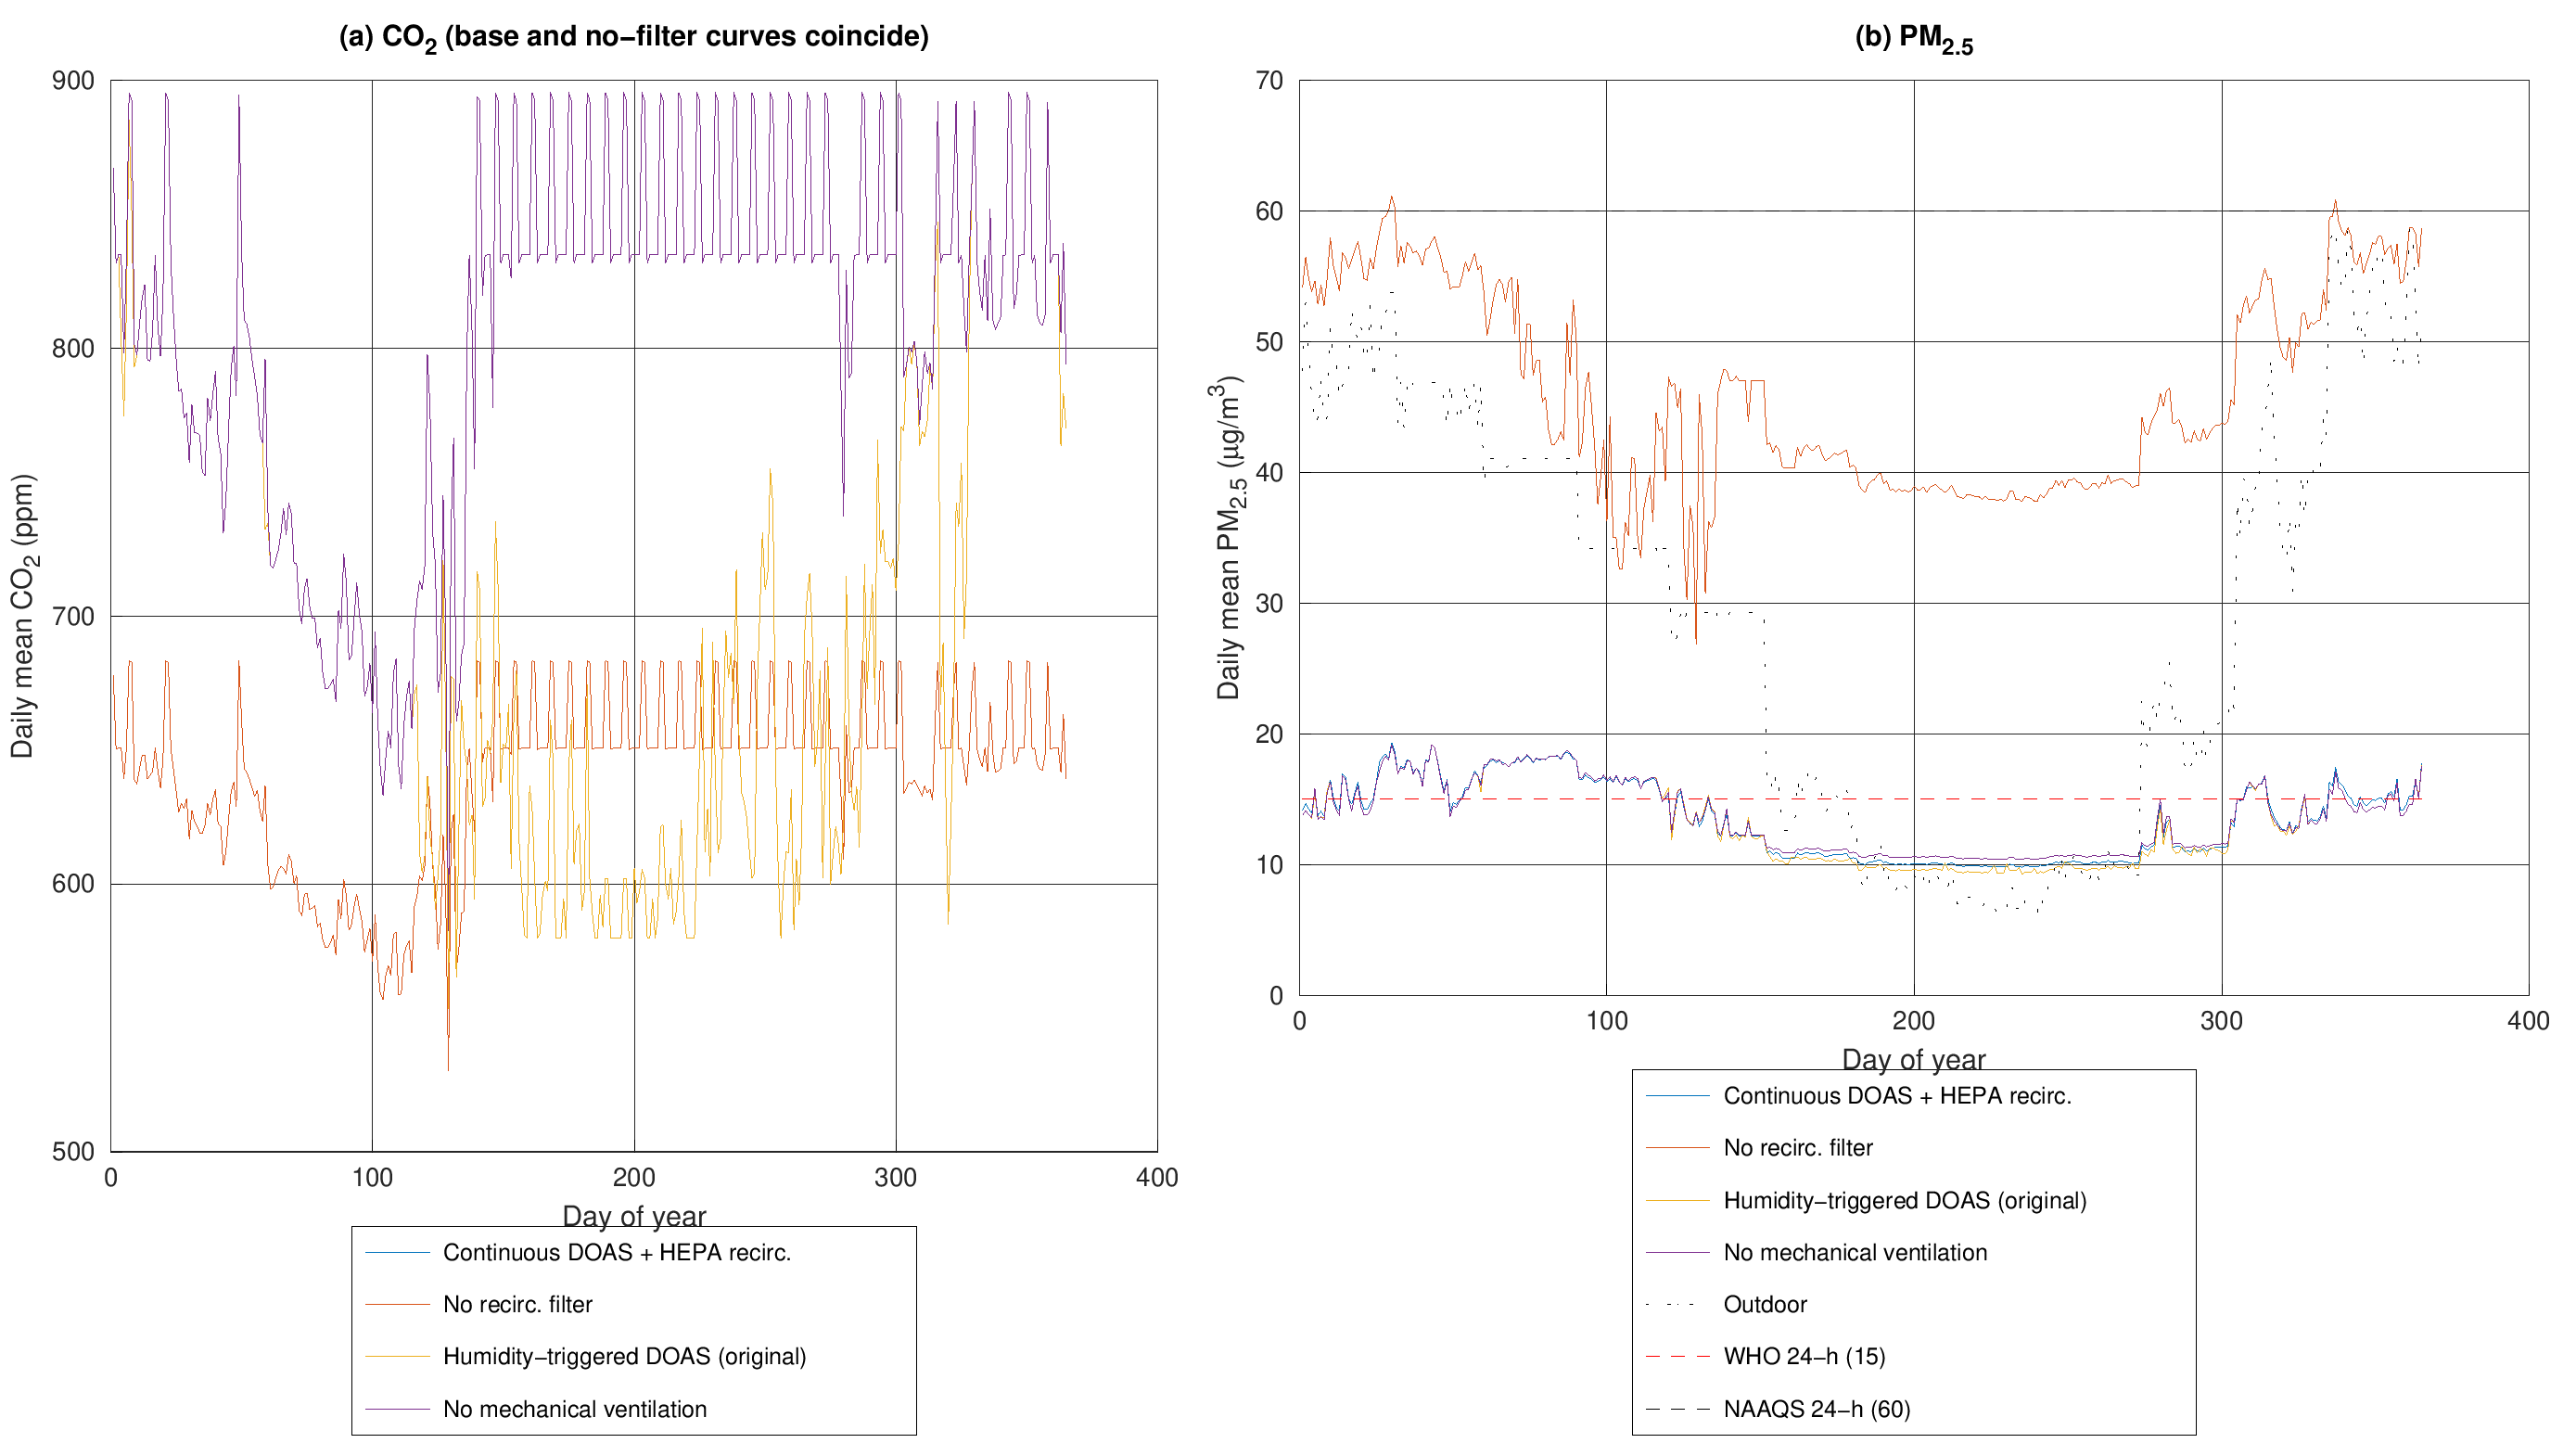
\includegraphics[width=\linewidth]{Fig07_iaq.png}
\caption{Daily mean indoor CO$_2$ (a) and PM$_{2.5}$ (b) for four ventilation and
filtration architectures (Hybrid controller).}\label{fig:iaq}
\end{figure}

\subsection{Discussion and limitations}
Replacing on/off control with modulating control gives the largest single gain. It
improves comfort, cuts compressor starts and, with PID or the model-based controllers,
lowers peak demand by 18--20\,\%. Within the modulating group, the Hybrid keeps the
economic operating point of E-MPC and adds two corrections: the PI layer lowers cost and
the safety override protects comfort. The DQN is competitive only with a shield, and its
seed-to-seed spread is an order of magnitude larger than that of the model-based
controllers. As \cite{biemann2021,wanghong2020} also report, a single training run is
not a reliable estimate of DRL performance.

The study has several limitations. The plant is a reduced-order model that has not
been calibrated against measurements or cross-checked against a detailed engine such as
EnergyPlus \cite{crawley2001}; we release an EnergyPlus case with identical inputs for
that check. Envelope, equipment and occupancy data are assumed, and the outdoor
PM$_{2.5}$ series is representative rather than measured. Comfort is judged by a static
dry-bulb band rather than an adaptive model \cite{manu2016}. Controller weights were
tuned on the evaluation year, so margins for an unseen year may be slightly smaller.
Finally, the mechanism tests are single-seed, and differences below about 0.5\,\%
should be read as ties.

\section{Conclusion and Future Work}\label{sec:conclusion}
We benchmarked five residential cooling controllers over a full year and five seeds
for a Pune apartment, with plant--model mismatch, sensor noise and forecast error
included. Under the base tariff the thermostat is cheapest but overcools. Among
controllers that deliver good comfort, the hierarchical Hybrid (E-MPC with a PI layer
and a safety override) performs best: it is \RelHybPidCost\,\% cheaper than PID with
\RelHybPidKh\,\% less discomfort. It remained the most comfortable controller under a
+3\,K heatwave, changes in thermal mass, three alternative tariffs and a 40-sample
variation of assumed inputs. The size of its saving, however, depends on the building,
and under the flat and utility tariffs the DQN was marginally cheaper.
The ablations show that E-MPC's comfort loss under heat comes from its narrow margin
rather than from prediction error, and that the Hybrid's cost gain comes from the PI
layer and most of its comfort gain from the safety override. A 1.7:1 ToD ratio produces
little load shifting, because peak-hour cooling serves occupied rooms and coincides with
heat release from the slab; a 3.6:1 ratio shifts about 5 percentage points of cooling
energy. Indoor air quality depends on ventilation and filtration design and is nearly the same
for all thermal controllers. Future work will cross-validate
the plant against EnergyPlus and field data, add measured PM$_{2.5}$ and adaptive,
humidity-aware comfort metrics, and co-optimize ventilation and cooling in a single
predictive controller.
